\setlength{\columnsep}{3pt}
\begin{flushleft}
	\textbf{Transmitting the data in the form of packets} over the internet is called casting.
	\newline
	\bigskip
	Let's see types of casting:
	\begin{figure}[h!]
		\centering
		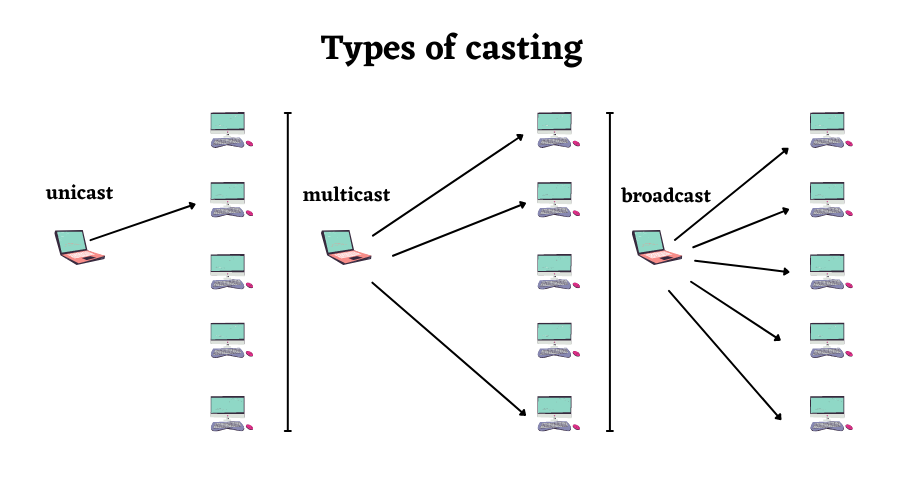
\includegraphics[scale=0.6]{content/chapter14/images/casting.png}
		\caption{Casting types}
		\label{fig:casting_types}
	\end{figure}

	\begin{itemize}
		\item \textbf{Unicast}: 
		\begin{itemize}
			\item \textbf{Transmitting data from one source host to one destination host} is called as unicast.
			\item It is a \textbf{one to one} transmission.
		\end{itemize}
	\item \textbf{Broadcast}: 
	\begin{itemize}
		\item \textbf{Transmitting data from one source host to all other hosts} residing in the same or other network is called as broadcast.
		\item It is a \textbf{one to all} transmission.
	\end{itemize}
	\item \textbf{Multicast}: 
	\begin{itemize}
		\item \textbf{Transmitting data from one source host to a particular group of hosts} having interest in receiving the data is called as multicast.
		\item It is a \textbf{one to many} transmission.
	\end{itemize}

	\end{itemize}


\end{flushleft}
\newpage


